% ============================================================
% Illustration: cross-extractor un-scaling + per-dataset re-z-scoring (SFM)
% Compile standalone -> fig_unscaling_scheme.pdf, place in figure-q1/.
% Answers reviewer: "add a simple diagram of how unscaling and
% re-z-scoring is done between the two extractors."
% ============================================================
\documentclass[tikz,border=6pt]{standalone}
\usepackage{helvet}\renewcommand{\familydefault}{\sfdefault}
\usepackage{amsmath}
\usepackage{tikz}
\usetikzlibrary{arrows.meta,positioning,fit,backgrounds}
\begin{document}
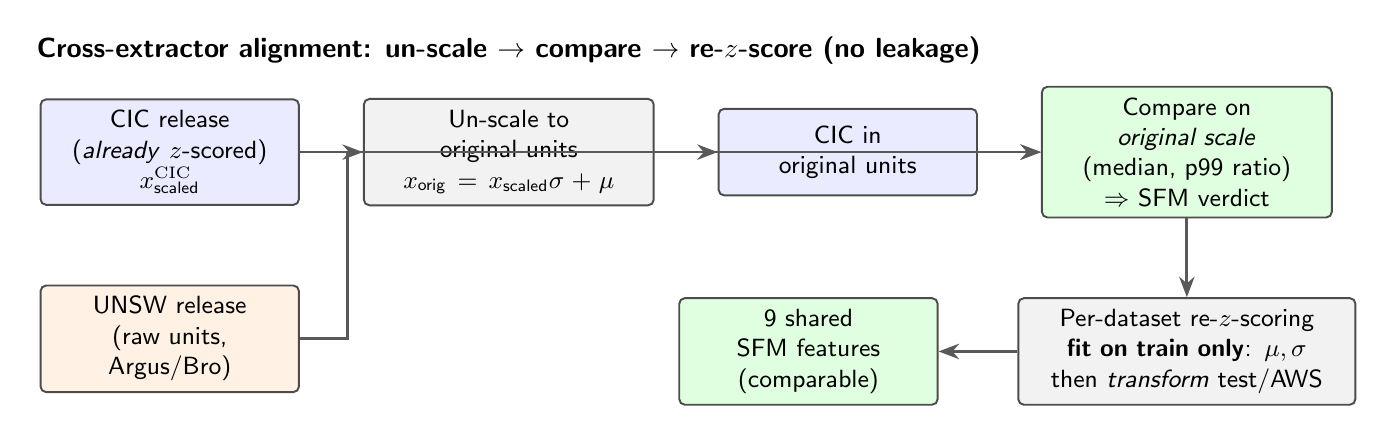
\begin{tikzpicture}[
  font=\small, >={Stealth[length=2.6mm]},
  b/.style={rounded corners=2pt, draw=black!70, line width=0.7pt, align=center,
            inner sep=4pt, minimum height=11mm, text width=30mm},
  cic/.style={b, fill=blue!8}, uns/.style={b, fill=orange!10},
  op/.style={b, fill=black!5, text width=34mm},
  shared/.style={b, fill=green!12, text width=34mm},
  a/.style={->, line width=1pt, draw=black!65},
]

% CIC branch (already z-scored on release) -> un-scale -> original units
\node[cic] (cicz) {CIC release\\(\emph{already} $z$-scored)\\$x^{\mathrm{CIC}}_{\text{scaled}}$};
\node[op, right=8mm of cicz] (uns1) {Un-scale to\\original units\\
  $x_{\text{orig}}=x_{\text{scaled}}\sigma+\mu$};
\node[cic, right=8mm of uns1] (cico) {CIC in\\original units};

% UNSW branch (raw)
\node[uns, below=10mm of cicz] (unsraw) {UNSW release\\(raw units,\\Argus/Bro)};

% Comparison on original scale (SFM verdict)
\node[shared, right=8mm of cico] (cmp) {Compare on\\\emph{original scale}\\
  (median, p99 ratio)\\$\Rightarrow$ SFM verdict};

% Per-dataset re-z-scoring, fit on TRAIN only
\node[op, below=10mm of cmp, text width=40mm] (rez)
  {Per-dataset re-$z$-scoring\\
   \textbf{fit on train only}: $\mu,\sigma$\\
   then \emph{transform} test/AWS};
\node[shared, left=10mm of rez, text width=30mm] (model) {9 shared\\SFM features\\(comparable)};

\draw[a] (cicz) -- (uns1);
\draw[a] (uns1) -- (cico);
\draw[a] (cico) -- (cmp);
\draw[a] (unsraw.east) -- ++(0.6,0) |- (cmp.west);
\draw[a] (cmp) -- (rez);
\draw[a] (rez) -- (model);

\node[font=\bfseries, above=3mm of uns1] {Cross-extractor alignment: un-scale $\to$ compare $\to$ re-$z$-score (no leakage)};
\end{tikzpicture}
\end{document}
